\phantomsection\label{eq:3-13}
\begin{equation}
\text{面积}=(n-1)\sqrt{s_{11}}\sqrt{s_{22}}\sqrt{1-r_{12}^{2}}=(n-1)\sqrt{s_{11}s_{22}(1-r_{12}^{2})}
\tag{3-13}
\end{equation}
又
\phantomsection\label{eq:3-14}
\begin{equation}
\begin{aligned}
|\mathbf{S}|&=\begin{vmatrix}s_{11}&s_{12}\\s_{12}&s_{22}\end{vmatrix}
=\begin{vmatrix}s_{11}&\sqrt{s_{11}}\sqrt{s_{22}}r_{12}\\[4pt]\sqrt{s_{11}}\sqrt{s_{22}}r_{12}&s_{22}\end{vmatrix}\\[6pt]
&=s_{11}s_{22}-s_{11}s_{22}r_{12}^{2}=s_{11}s_{22}(1-r_{12}^{2})
\end{aligned}
\tag{3-14}
\end{equation}
如果我们比较\hyperref[eq:3-14]{式(3-14)} 和\hyperref[eq:3-13]{式(3-13)}, 可见
\[
|\mathbf{S}|=(\text{面积})^{2}/(n-1)^{2}
\]
对于由 $p-1$ 个偏差向量 $\mathbf{d}_{1},\mathbf{d}_{2},\cdots,\mathbf{d}_{p-1}$ 所产生的 $n$ 维空间的体积, 假定 $|\mathbf{S}|=(n-1)^{-(p-1)}(\text{体积})^{2}$ 成立, 那么, 对于 $p$ 个偏差向量, 由归纳法, 我们可以确定以下一般性的结论 (参见文献 [1]):
\phantomsection\label{eq:3-15}
\begin{equation}
\text{广义样本方差}=|\mathbf{S}|=(n-1)^{-p}(\text{体积})^{2}
\tag{3-15}
\end{equation}
\hyperref[eq:3-15]{式(3-15)} 说明, 对于一个固定的数据集合, 广义样本方差是与由 $p$ 个偏差向量\footnote{如果广义方差是用样本协方差矩阵 $\mathbf{S}_{n}=[(n-1)/n]\mathbf{S}$ 定义, 则利用结论 2A.11, $|\mathbf{S}_{n}|=|[(n-1)/n]\mathbf{I}_{p}||\mathbf{S}|=[(n-1)/n]^{p}|\mathbf{I}_{p}||\mathbf{S}|=[(n-1)/n]^{p}|\mathbf{S}|$. 因此, 利用\hyperref[eq:3-15]{式(3-15)}, 我们也可以有: 广义样本方差 $=|\mathbf{S}_{n}|=n^{-p}(\text{体积})^{2}$.} $\mathbf{d}_{1}=\mathbf{y}_{1}-\bar{x}_{1}\mathbf{1}$, $\mathbf{d}_{2}=\mathbf{y}_{2}-\bar{x}_{2}\mathbf{1},\cdots,\mathbf{d}_{p}=\mathbf{y}_{p}-\bar{x}_{p}\mathbf{1}$ 生成的体积的平方成比例的. \hyperref[fig:3.6]{图 3.6}(a) 和 (b) 指出了由 $p=3$ 所对应的“大的”和“小的”广义方差的剩余向量生成的梯形区域.

\begin{center}
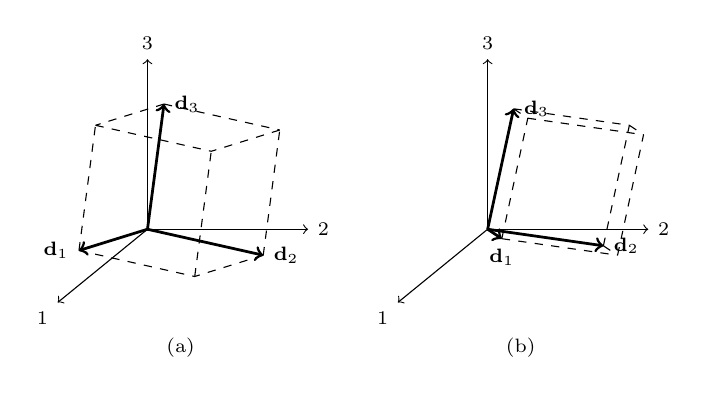
\begin{tikzpicture}[scale=0.60]
% ===== (a) 大的广义样本方差 =====
\begin{scope}
\draw[->] (0,0)--(3.4,0) node[right,font=\scriptsize]{$2$};
\draw[->] (0,0)--(0,3.6) node[above,font=\scriptsize]{$3$};
\draw[->] (0,0)--(-1.9,-1.55) node[below left,font=\scriptsize]{$1$};
\coordinate (O) at (0,0);
\coordinate (A) at (-1.45,-0.45);
\coordinate (B) at (2.45,-0.55);
\coordinate (C) at (0.35,2.65);
\coordinate (D) at (1.00,-1.00);
\coordinate (E) at (-1.10,2.20);
\coordinate (F) at (2.80,2.10);
\coordinate (G) at (1.35,1.65);
\draw[->,line width=1.0pt] (O)--(A) node[left,font=\scriptsize]{$\mathbf{d}_{1}$};
\draw[->,line width=1.0pt] (O)--(B) node[right,font=\scriptsize]{$\mathbf{d}_{2}$};
\draw[->,line width=1.0pt] (O)--(C) node[right,font=\scriptsize]{$\mathbf{d}_{3}$};
\draw[dashed] (A)--(D) (B)--(D) (A)--(E) (C)--(E) (B)--(F) (C)--(F) (D)--(G) (E)--(G) (F)--(G);
\node[font=\scriptsize] at (0.7,-2.5){(a)};
\end{scope}
% ===== (b) 小的广义样本方差 =====
\begin{scope}[shift={(7.2,0)}]
\draw[->] (0,0)--(3.4,0) node[right,font=\scriptsize]{$2$};
\draw[->] (0,0)--(0,3.6) node[above,font=\scriptsize]{$3$};
\draw[->] (0,0)--(-1.9,-1.55) node[below left,font=\scriptsize]{$1$};
\coordinate (O2) at (0,0);
\coordinate (A2) at (0.55,2.55);
\coordinate (B2) at (2.45,-0.35);
\coordinate (C2) at (0.30,-0.20);
\coordinate (D2) at (3.00,2.20);
\coordinate (E2) at (0.85,2.35);
\coordinate (F2) at (2.75,-0.55);
\coordinate (G2) at (3.30,2.00);
\draw[->,line width=1.0pt] (O2)--(A2) node[right,font=\scriptsize]{$\mathbf{d}_{3}$};
\draw[->,line width=1.0pt] (O2)--(B2) node[right,font=\scriptsize]{$\mathbf{d}_{2}$};
\draw[->,line width=1.0pt] (O2)--(C2) node[below,font=\scriptsize]{$\mathbf{d}_{1}$};
\draw[dashed] (A2)--(E2) (C2)--(E2) (B2)--(F2) (C2)--(F2) (A2)--(D2) (B2)--(D2) (E2)--(G2) (F2)--(G2) (D2)--(G2);
\node[font=\scriptsize] at (0.7,-2.5){(b)};
\end{scope}
\end{tikzpicture}
\end{center}

\begin{center}
\phantomsection\label{fig:3.6}{\zihao{6}\heiti 图 3.6}\\[2pt]
{\zihao{6} (a) 对 $p=3$, “大的”广义样本方差}\\[2pt]
{\zihao{6} (b) 对 $p=3$, “小的”广义样本方差}
\end{center}

对于一个固定大小的样本, 根据几何学, 当任何 $\mathbf{d}_{i}=\mathbf{y}_{i}-\bar{x}_{i}\mathbf{1}$ (或 $\sqrt{s_{ii}}$) 的长度增加时, 明显地体积或 $|\mathbf{S}|$ 也增加. 另外, 如果移动固定长度的剩余向量直到它们互相成直角为止时, 体积也将增加, 如\hyperref[fig:3.6]{图 3.6}(a). 另一方面, 如果仅仅 $s_{ii}$ 的一个是小的, 或者偏差向量之一几乎在由其他向量或两个向量构成的 (超) 平面中时, 体积或 $|\mathbf{S}|$ 将是小的. 在第二种情况中, 不规则四边形在平面上有很小的高. 这情况如\hyperref[fig:3.6]{图 3.6}(b) 所示, 其中 $\mathbf{d}_{1}$ 几乎在由 $\mathbf{d}_{2}$ 和 $\mathbf{d}_{3}$ 所构成的平面内.

在 $p$ 维空间广义方差也有解释, 即数据的散布图表示法. 大多数直观的解释涉及关于样
